 \documentclass[12pt]{article}
\usepackage[T2A]{fontenc}
\usepackage[utf8]{inputenc}       

\usepackage[russian, english]{babel}
\usepackage{amsmath,amsfonts,amsthm,amssymb,amsbsy,amstext,amscd,amsxtra,multicol}
\usepackage{verbatim}
\usepackage{tikz}
\usetikzlibrary{automata,positioning}
\usepackage{multicol}
\usepackage{graphicx}
\usepackage[colorlinks,urlcolor=blue]{hyperref}
\usepackage[stable]{footmisc}
\usepackage{ dsfont }
\usepackage{wrapfig}
\usepackage{xparse}
\usepackage{ifthen}
\usepackage{bm}
\usepackage{color}
 \usepackage{subfigure}
 
\usepackage{algorithm}
\usepackage{algpseudocode}

\usepackage{xcolor}
\usepackage{hyperref}
\definecolor{linkcolor}{HTML}{799B03} % цвет гиперссылок
\definecolor{urlcolor}{HTML}{799B03} % цвет гиперссылок
 
%\hypersetup{pdfstartview=FitH,  linkcolor=linkcolor,urlcolor=urlcolor, colorlinks=true}

\newtheorem{theorem}{Теорема}[section]
\newtheorem{lemma}{Лемма}[section]

\DeclareMathOperator{\sign}{sign}
\DeclareMathOperator{\grad}{grad}
\DeclareMathOperator{\intt}{int}
\DeclareMathOperator{\conv}{conv}
\begin{document}

\tableofcontents
\newpage


\section{Описание метода}

Рассмторим задачу минимизации функции от двух переменных, заданной на квадрате:

$$\min_{(x,y)}\left\{f(x,y)|(x,y) \in Q\right\},$$
где $f$ - это выпуклая функция, $Q$ - квадрат на плоскости. Здесь и далее будем считать, что стороны квадрата соориентированы параллельно осям текущей системы координат. Очевидно, что это не предположение не существенно, поскольку для любого квадрата существует тривиальное афинное преобразование, которое повернет этот квадрат так, чтобы он соответствовал условию

Тогда рассмотрим метод двумерной дихотомии. Его основные этапы следующие:

1. Провести отрезок через центр квадрата параллельно оси Ox.

2. Решить одномерную задачу оптимизации на этом отрезке с некоторой точностью $\delta$

3. Вычислим градиент в полученной точке и отбросим прямоугольник, в который смотрит этот градиент

4. Повторить шаги 2-3 для вертикального отрезка через центр

5. Повторять шаги 1-4, пока не достигнута необходимая точность по функции.

Заметим, что на шаге 3 мы не нуждаемся во всем градиенте, а только в его ортогональной компоненте, т.е. производной по той переменной, которая была фиксировона на текущем отрезке.

Для решения одномерной задачи мы можем использовать любой метод одномерной оптимизации. Однако, в следующих разделах мы покажем, что дифференцируемость функции - существенное условие для сходимости метода, поэтому без ограничения общности мы можем и будем использовать метод дихотомии, использующий производную в центре отрезка, поскольку этот метод гарантирует линейную скорость сходимости и при этом является одноточечным, в отличии, например, от метода золотого сечения или метода дихотомии нулевого порядка.

Утверждается, что для некоторой точности решения вспомогательной задачи $\delta$ данный метод будет сходиться к решению по функции. Это будет обсуждено в следующей секции.

Сейчас обсудим корректность алгоритма. Здесь и далее мы будем использовать следующую нотацию. Если у нас определен некоторый сегмент и есть некоторый вектор $\textbf{g}$, то $\textbf{g}_\parallel$ - его проекция на этот отрезок, а $\textbf{g}_\perp$ - его перпендикулярная компонента.

Здесь и далее нам понадобятся стандартные понятия субдифференциала и субградиента, которые можно найти, например, в \cite{Nesterov}.

Нам понадобится следующая лемма.

\begin{lemma}
\label{subgradient}

Если $\textbf{x}_*$ решение одномерной задачи оптимизации:

$$\exists g \in \partial_Q f(\textbf{x}_*) : g_\parallel = 0$$
\end{lemma}
\begin{proof}[Доказательство]
Если $\textbf{x}_*$ есть внутренняя точка, то производная по нефиксированной переменной равна нулю в силу того, что $\textbf{x}_*$ - минимум. Тогда с учетом того, что $\nabla f(\textbf{x}_*)\in\partial f(\textbf{x}_*)$, получаем утвержение из теоремы.

Допустим, что $\textbf{x}_*$ граничная точка. Тогда множество условного субдифференциала на квадрате $Q$ определяется следующим образом:

$$\partial_Q f(\textbf{x}) = \partial f(\textbf{x}) + N\left(\textbf{x}|Q\right),$$
где $N(\textbf{x}|Q) = \left\{\textbf{a}|\langle\textbf{a}, \textbf{y} - \textbf{x}\rangle\leq 0, \forall \textbf{y} \in Q\right\}$. 

Далее предполагаем, что мы решаем задачу оптимизации на горизонтальном сегменте и $\textbf{x}_*$ есть правый конец этого отрезка. Доказательство на три других случая (другой конец горизонтального сегмента и два конца вертикального сегмента). В нашем случае:

$$\partial f(\textbf{x}_*) = \{\nabla f(\textbf{x}_*)\},$$
$$N(\textbf{x}|Q) =\left\{\textbf{a}|\textbf{a}_\perp = 0, \textbf{a}\parallel \geq0\right\}$$

Заметим, что $\left(\nabla f(\textbf{x}_*)\right)_\parallel \leq 0$, потому что, если бы это было не так, то очевидно $\textbf{x}_*$ - не минимум функции $f$ на этом сегменте. Тогда выбрав $\textbf{a}$, такой что $\textbf{a}_\parallel = -\left(\nabla f(\textbf{x}_*)\right)_\parallel$, получаем субградиент из условия:

$$\textbf{g} = \nabla f(\textbf{x}_*) + \textbf{a} : \textbf{g}_\parallel =0$$
\end{proof}

\begin{theorem}
Если функция $f$ выпуклая непрерывно дифференцируемая функция, то для решения  любой одномерной задачи существует некоторая его окрестность, такая что, если выбрать прямоугольник на основе перпендикулярной компоненты градиента в любой точке этой окрестности, выбор будет такой же, как и в случае использования градиента в точке-решении.
\end{theorem}

Данный метод работает не для всех выпуклых функций, даже если решать задачу одномерной оптимизации точно. Пример негладкой выпуклой функции был расмотрен в \cite{Ston_Pas}.

\section{Одномерная задача}
\label{Delta}

В этой секции мы опишем достаточную точность решения вспомогательной задачи на отрезке. Мы будем использовать следующие обозначения:

$$(x_*,y_*) \text{ or }\textbf{x}_*\text{ -- solution of one-dimensional problem} $$
$$\delta = |x-x_*| \text{ -- distance}$$

В работе \cite{Ston_Pas} была доказана следующая теорема:

\begin{theorem}
\label{ConstEst}
Пусть функция $f$ выпуклая и удовлетворяет условие Липшица с константой $M$, а ее градиент - с константой $L$.
Тогда если каждая одномерная задача решена со следующей точностью по аргументу
\begin{equation}
\delta \leq \frac{\epsilon}{2La(\sqrt{2}+\sqrt{5})(1-\frac{\epsilon}{Ma\sqrt{2}})}
\end{equation}
то метод двумерной дихотомии сходится к решению с точностью $\epsilon$ по функции.
\end{theorem}

Данная стратегия всегда требует решать задачу с точностью порядка $\epsilon$. А также данный метод может не гарантировать сходимости по аргументу. Такой пример также был рассмотрен в работе \cite{Ston_Pas}. Далее мы будем называть эту стратегию \textbf{ConstEst}(Constant Estimate).

Теперь разработаем стратегию, которая гарантирует сходимость по аргументу. Заметим, что прямоугольник выбирается правильно, если знак производной в решении вспомогательной задачи совпадает со знаком производной в ее приближении:

\begin{equation}\label{MCH}
f'_\perp(\textbf{x}_*)f'_\perp(\textbf{x}_*+\delta) > 0
\end{equation}

Здесь и далее мы будем использовать следующую простую лемму:

\begin{lemma}
\label{trick_lemma}
$\forall a,b\in\mathbb{R}\backslash\{0\}, |a-b|\leq |b| \Rightarrow \sign a = \sign b$
\end{lemma}
\begin{proof}[Доказательство]
Если $b>0$ и $a\leq b$, тогда условие из леммы эквивалентно следующему:
$$b-a\leq b\Rightarrow a\geq 0.$$
Если $b>0$ и $a \geq b$, тогда $a\geq 0$.

Случай отрицательного $b$ доказывается аналогично.
\end{proof}

\begin{theorem}
\label{CurGrad}
Пусть функция $f$ выпуклая с липшецевым градиентом с константой $L$. Точка $\textbf{x}_*$ решение одномерной задачи оптимизации, $\textbf{x}$ - ее приближение.

Тогда если приближение удовлетворяет следующему условию:

$$\delta \leq \frac{|f_\perp'(\textbf{x})|}{L},$$
то прямоугольник, выбранный на основе градиента в этой точке, содержит решение исходной задачи на квадрате. 
\end{theorem}
\begin{proof}[Доказательство]

Из леммы \ref{trick_lemma} следует, что для того чтобы совпали знаки, достаточно потребовать

$$\left|f'_\perp(\textbf{x}_*) - f'_\perp(\textbf{x})\right| \leq |f'_\perp(\textbf{x})|$$

Используя липшецевость градиента получаем утверждение теоремы.
\end{proof}

Описанная в теореме оценка крайне не эффективна, если модуль перпендикулярной компоненты стремительно убывает при приближении к точке-решению, поэтому сформулируем альтернативное условие остановки:

\begin{theorem}
\label{small}
Пусть $f$ есть $M$-липшецева выпуклая с $L$-липшецевым градиентов. Точка $\textbf{x}_*$ есть решение одномерной задачи оптимизации, $\textbf{x}$ - ее приближение, $\delta = \|\textbf{x}_*-\textbf{x}\|$ - верхняя оценка расстояния между ними.

Тогда для достижения точности $\epsilon$ в точке $\textbf{x}$ следующего условия достаточно:
$$\delta \leq \frac{\epsilon-LR|f_\perp'(x)|}{L+MR}, $$
where $R=a\sqrt{2}$ is size of current square.
\end{theorem}

\begin{proof}[Доказательство]

Из леммы \ref{subgradient} мы имеем:

$$g \in \partial f(\textbf{x}_*): g_\parallel = 0.$$

Then the following inequallity is true by diffenition of subgradient:

Тогда по определению субградиента:

$$f(\textbf{x}^*) - f(\textbf{x}_*) \geq (g, \textbf{x}^* - \textbf{x}_*)$$

Используем неравенство Коши-Буняковского-Шварца:
$$f(\textbf{x}_*) - f(\textbf{x}^*) \leq -(g, \textbf{x}^* - \textbf{x}_* )\leq$$
$$\leq \|g\| \|\textbf{x}^* - \textbf{x}_*\|\leq \|g\|a\sqrt{2}$$

С другой стороны, из липшецевости функции мы имеем:
$$f(\textbf{x})-f(\textbf{x}_*)\leq M\delta$$

$$f(\textbf{x})-f(\textbf{x}^*) \leq M\delta +\|g\|a\sqrt{2} = M\delta + |f_\perp'(\textbf{x}_*)|R$$

Из липшецевости градиента:
$$f(\textbf{x})-f(\textbf{x}^*) \leq M\delta + \left(|f_\perp'(\textbf{x})|+L\delta\right)R$$

Тогда для достижения точности $\epsilon$ по функции в точке $\textbf{x}$ для исходной задачи достаточно следующего условия:

$$M\delta +\|g\|a\sqrt{2} = M\delta + \left(|f_\perp'(\textbf{x})|+L\delta\right)R \leq \epsilon$$

$$\delta \leq \frac{\epsilon - |f_\perp'(\textbf{x})|}{M+LR}$$
\end{proof}

Then our addaptive strategy is following. One is to calculate untill the following condition is met:

Определим нашу адаптивную стратегию. Мы решаем задачу одномерной оптимизации, пока не выполнено условие на точность по аргументу:

\begin{equation}
\label{Adaptive}
\delta \leq \max\left\{
	\frac{|f_\perp'(\textbf{x})|}{L}, 
	\frac{\epsilon - |f_\perp'(\textbf{x})|}{M+LR}
	\right\}.
\end{equation}

Причем, если выполнено условие из теоремы \ref{small}, мы останавливаем весь метод. Эту стратегию мы назвали \textbf{CurGrad}(Current Gradient).


\section{Сходимость}

В этой сецкии будут приведены оценки для количества итераций глобального метода для достижения точности по функции. В данном разделе под итерацией подразумевается одна итерация метода двумерной дихотомии, в результате которой квадрат уменьшается вдвое.

\begin{theorem}
Если функция $f$ выпуклая и $Ь$-липшецева, тогда для достижения $\epsilon$ по функции следующего количества итераций достаточно:
\begin{equation}\label{NI1}N = \left\lceil\log_2\frac{\sqrt{2}Ma}{\epsilon}\right\rceil\end{equation}
где $a$ размер исходного квадрата $Q$.
\end{theorem}

Доказательство для стратегии \textbf{ConstEst} было проведено в работе \cite{StonPas}. Для стратегии \textbf{CurGrad} данная оценка есть очевидное следствие липшецевости функции и сходимости по аргументу.

Однако мы можем улучшить нашу оценку, если учтем сходимость по аргументу.
\begin{theorem}
Пусть $f$ - выпуклая функция.

Если

1. Функция $f$ имеет $L$-липшецев градиент

2. $\exists \textbf{x}^*\in Q: \nabla f(\textbf{x}^*) = \textbf{0}$

3. Стратегия для решения одномерной задачи обеспечивает сходимость по аргументу

тогда для достижения точности $\epsilon$ по функции следующего количества итераций достаточно:
\begin{equation}\label{NI3}N = \left\lceil\frac{1}{2}\log_2\frac{La^2}{4\epsilon}\right\rceil,
\end{equation}
где $a$ - размер исходного квадрата $Q$.
\end{theorem}

\begin{proof}[Доказательство]
Для всех выпуклых дифференцируемых функций следующее неравенство верно (доказательство можно найти в \cite{Nesterov}):
$$f(\textbf{x}) - f(\textbf{x}^*) - (f'(\textbf{x}^*), \textbf{x} - \textbf{x}^*) \leq \frac{L}{2}\|\textbf{x}-\textbf{x}^*\|^2$$

По условию теоремы существует такая точка $\textbf{x}^*$, что $f'(\textbf{x}^*) = 0$. Заметим, что эта точка является решением задачи. Тогда наше неравенство примет вид:

$$f(\textbf{x}) - f(\textbf{x}^*)\leq \frac{L}{2}\|\textbf{x}-\textbf{x}^*\|^2$$

После $N$ итераций имеем следующую оценку:

$$f(\textbf{x}) - f(\textbf{x}^*)\leq L\left(\frac{a}{2^N}\right)^2,$$
что доказывает оценку из теоремы.
\end{proof}


\section{Двойственные задачи}
\label{details}

Данный метод предполагает особый интерес в приложении решения двойственных задач для задач с двумя ограничениями. А именно, для решения задач вида:

\begin{gather}
\phi(\lambda_1, \lambda_2) \rightarrow \min_{\lambda\geq 0},\\
\text{where } \phi = -\min_\textbf{x}\left(f(\textbf{x}) + \lambda_1 g_1(\textbf{x}) + \lambda_2 g_2(\textbf{x})\right)
\end{gather}
$$\textbf{x}(\lambda) = \arg\min_\textbf{x}\Phi(\textbf{x}, \lambda)$$

In this section we will discuss how transform this task to task of the task of minimization on square, what is derivative and lipschitz constants. Also, there is description of way for to calculate the value of function $\phi$ and its derivative.

В данной секции мы обсудим как свести это к нашей задаче, как вычислить липшецевы константы и каким образом вычислять $\textbf{x}(\lambda)$.

Для начала приведем задачу к задаче минимизации на квадрате. Согласно \cite{task} (see ex. 4.1), мы имеем следующую локализацию на решение:

\begin{gather}
\label{restr:dual}
\|{\lambda}\|_1 \leq a = \frac{1}{\gamma}\left(f(\overline{\textbf{x}}) -\min\limits_{\textbf{x}}f(\textbf{x})\right),\\
\text{where $\overline{\textbf{x}}:g_i(\overline{\textbf{x}})<0,\gamma = \min\limits_i[-g_i(\overline{\textbf{x}})]$}
\end{gather}
Согласно этому утверждению, мы можем локализовать $\lambda^*$ в квадрате $Q = [0, a]^2$. В таком случае мы свели нашу задачу оптимизации к следующему виду:
\begin{gather}
\label{dual}
\phi(\lambda_1, \lambda_2) \rightarrow \min_{\lambda \in Q}
\end{gather}

Градиент функции $\phi$ мы будем считать согласно хорошо известной теорема Демьянова-Данскина-Рубинова, см. \cite{DDR-theorem}.

\begin{theorem}
Пусть $\phi(\lambda)=\min\limits_{x\in X}\Phi(x,\lambda)$ для всех $\lambda\geq0$, где $\Phi$ это гладкая выпуклая функция по $\lambda$. Тогда
$$\nabla \phi(\lambda) = F'_\lambda\left(x(\lambda),\lambda\right)$$
\end{theorem}

Условия теоремы выполнено в нашем случае и мы получаем:
\begin{equation}
\phi'_{\lambda_k}(\lambda) = g_k\left(\textbf{x}(\lambda)\right)
\end{equation}

Кроме этого, мы нуждаемся в константе Липшица для градиента. В работе \cite{Stonykin} сформулирована и доказана следующая теорема:
\begin{theorem}
Let $f(x)$ be a $\mu_f$-strongly convex function, the function $g(x)$ satisfies the Lipschitz condition with a constant $M_g$. Then the function $\phi(\lambda) = \min_\textbf{x}\left(f(\textbf{x}+\lambda_1g_1(\textbf{x}) + \lambda_2g_2(\textbf{x})\right)$ defined in \ref{phi}, where $x(\lambda) = \arg\min\limits_x(f(x)+\lambda g(x))$, has Lipschitz smooth gradient with constant $L_{\phi'} = \frac{M_g^2}{\mu_f}$
\end{theorem}

В случае размерности 2 по $\lambda$ доказательство повторяется практически в точности. В таком случае, $g(\textbf{x})$ есть вектор-функция.

Основная сложность решения седловых задач есть то, что вычисление $\textbf{x}(\lambda)$ точно в большинстве случаев невозможно. Следовательно, мы не имеем доступа к точному значению градиента. Это приводит к следующим проблемам:

1. Шаг дихотомии на отрезке

2. Проверка стоп-условия из стратегии \textbf{CurGrad}

3. Выбор прямоугольника

Заметим, что нас в каждой из задач интересуют следующие величины:

1. Проекция градиента на отрезок, т.е. $g_\parallel(\textbf{x}(\lambda))$.

2. Значение разниц $\delta-\frac{|g_\perp(\textbf{x}(\lambda))|}{L}$ и $\delta-...$, где $L$ это липшецева константа для градиента $\phi$.

3. Перпендикулярная компонента, т.е. $g_2(\textbf{x}(\lambda))$.

Согласно \cite{Ston_Pas}, мы можем вычислять производные неточно, для того чтобы выбрать прямоугольник с $\epsilon$-решением. Так, если $\delta$ - это точность по аргументу текущего приближения одномерной задачи, и $\Delta$ - точность вычисления градиента в точке по величине градиента, то следующего условия достаточно для нужного выбора прямоугольника:

$$2\Delta + L\delta \leq \frac{\epsilon}{2a(\sqrt{2}+\sqrt{5})},$$
где $L$ - это липшецева константа градиента для двойственной задачи. Мы можем увидеть, что задача выбора сегмента с решением одномерной задачи является одномерным вариантом той же проблемы. Это приводит нас к следующей теореме.

\begin{theorem}
\label{StonPas_Dual}
Если одномерная задача решается со следующей точностью $delta =  \frac{\epsilon}{4La(\sqrt{2}+\sqrt{5})}$ по аргументо, тогда, для того чтобы выбрать прямоугольник с $\epsilon$-решением, достаточно вычислять $\textbf{x}(\lambda)$ в текущей точке со следующей точностью:

\begin{equation}
\|\textbf{x} - \textbf{x}(\lambda)\| \leq \frac{1}{M_g}\frac{\epsilon}{8a(\sqrt{2}+\sqrt{5})}
\end{equation}

Для того, чтобы выбрать сегмент с решением одномерной задачи, достаточно вычислять $\textbf{x}(\lambda)$ в центре текущего сегмента со следующей точностью:
\begin{equation}
\|\textbf{x} - \textbf{x}(\lambda)\| \leq \frac{1}{M_g}\frac{\epsilon}{4a(\sqrt{2}+\sqrt{5})}
\end{equation}
\end{theorem}

С другой стороны, для каждого случая интересен только знак соответствующих выражений. Для этого мы будем применять  лемму \ref{trick_lemma}. Согласно этой лемме, мы имеем следующие достаточные условия для остановки вычисления $\textbf{x}(\lambda)$ для выше обозначенных случаев:

1. $|g_\parallel(\textbf{x})-g_\parallel(\textbf{x})|\leq |g_\parallel(\textbf{x})|$

2. $\frac{1}{L}\Big||g_\perp(\textbf{x})|-|g_\perp(\textbf{x}(\lambda))|\Big|\leq \Big|\delta-\frac{|g_\perp(\textbf{x})|}{L}\Big|$

3. $|g_\perp(\textbf{x})-g_\perp(\textbf{x}(\lambda))|\leq |g_\perp(\textbf{x})|$

Тогда сформулируем утверждения:

\begin{theorem}\label{x_lambda}
Пусть $g_k$ есть $L_{g_k}$-липшецевы функции. Тогда следующие утверждения верны.

1. Для того, чтобы сделать шаг дихотомии корректно, т.е. сохраняя сходимость по аргументу, достаточно вычислять $\textbf{x}(\lambda)$, пока не выполнено следующее условие
$$L_{g_\parallel}\|\textbf{x}-\textbf{x}(\lambda)\|\leq |g_\parallel(\textbf{x})|.$$

2. For to test stop condition correctly one can calculate $\textbf{x}(\lambda)$ untill the following condition is approache
2. Для того, чтобы проверить условие останова из стратегии 
$$\frac{L_{g_\perp}}{L}\|\textbf{x}-\textbf{x}(\lambda)\|\leq\Big|\delta-\frac{|g_\perp(\textbf{x})|}{L}\Big|,$$
where $\delta$ is a distance between $\lambda$ and solution of one dimensional task $\lambda_*$.

3. For to select rectangle according to strategy one can calculate $\textbf{x}(\lambda)$ untill the following condition is approached:
$$L_{g_\perp}\|\textbf{x}-\textbf{x}(\lambda)\|\leq |g_\perp(\textbf{x})|.$$
\end{theorem}

There are two interesting remarks.

Firstly, the calculating of $\textbf{x}(\lambda)$ does not depend on required accuracy $\epsilon$ for function $\phi$. This result is unique for our method and one can not see such effect in other inexact methods (see the next section).

Secondly, this strategies from written above theorem does not guarantee that the calculating of $\textbf{x}(\lambda)$ will stop. For example, let's consider the first condition. If $g_1(\textbf{x}(\lambda)) = 0$  and $|g_1(\textbf{x})|$ decreases faster than $L_{g_1}\|\textbf{x}-\textbf{x}(\lambda)\|$ with decreasing of $\|\textbf{x}-\textbf{x}(\lambda)\|$ than the stop condition will not be approached. This case is looked as extra specific and does not observed in our experiments but it can take place.



\section{Complexity}

Let's estimate complexity of one-dimensional problem.

For the strategy \textbf{ConstEst} we have that each one-dimensional problem needs exactly the following iterations of one-dimensional method:

$$\log_2\frac{2La(\sqrt{2}+\sqrt{5})(1-\frac{\epsilon}{Ma\sqrt{2}})}{\epsilon} = O\left(\log \frac{1}{\epsilon}\right)$$

Now let's condider the strategy \textbf{CurGrad}. Let the modul of the perpendicular component at point-solution $|f'_\perp(\textbf{x}_*)|$ is equal to $\tilde{\epsilon}$. A point from segment $\textbf{x}$ is its approximation and $\delta$ is a distance between them.

If we use the dichotomy method and $N$ is a number of current dichotomy iteration we have from $L$-Lipschitz continious gradient the following estimates for derivative at $\textbf{x}$:
$$\tilde{\epsilon}-La2^{-N} \leq |f_\perp'(\textbf{x})|\leq \tilde{\epsilon}+La2^{-N}$$

Accordint to this estimates for to approach a the first alternative from adaptive estimate \ref{Adaptive} the following condition is sufficient:

$$a2^{-N} \leq \frac{\tilde{\epsilon}-La2^{-N}}{L}$$

Similarly for the second alternative:

$$a2^{-N} \leq \frac{\epsilon - \tilde{\epsilon} - La2^{-N}}{M+LR}\leq \frac{\epsilon - \tilde{\epsilon}}{M+LR} - La2^{-N}$$

Accordint to this we have that for to approach estimate \ref{Adaptive} we need the following iterations number:

$$1+\log_2\min\left\{\frac{La}{\tilde{\epsilon}},\frac{(M+LR)a}{\epsilon-\tilde{\epsilon}}\right\}$$

Of course, we assume in this estimate that $\tilde{\epsilon}$ and $\epsilon-\tilde{\epsilon}$ are positive. If it is not true we can trash a bad alternative.

The bad case of this iterations number's estimate occurs when

$$\tilde{\epsilon} = \frac{L}{M+L(R+1)}\epsilon.$$

In the bad case we have the following estimate for iterations number:
$$1+\log_2\frac{(M+L(R+1))a}{\epsilon} = O\left(\log\frac{1}{\epsilon}\right)$$

From this estimate we see that the our adaptive strategy needs the same iterations number in the bad case as the strategy \textbf{ConstGrad} needs always.

But for complexity estimation we have that for to solve one-dimensional problem we needs $O\left(\log \frac{1}{\epsilon}\right)$ iterations.

\begin{theorem}
For to approach accuracy $\epsilon$ on function our method needs the following number of calculating function $f$ and its derivatives of the first order:
$$O\left(\log^2\frac{1}{\epsilon}\right)$$
\end{theorem} 
\begin{proof}[Доказательство]
We have that for to solve one-dimensional problem one needs not more than
$$\log_2\frac{Ca}{\epsilon}$$
iteration, where $C$ is a constant determined by the used strategy and function's parameter and $a$ is a size of current segment.

On each iteration of our method we solve to problems on segments of size $a_N=a2^{-N}$. Let $N_{\max1}=\left\lfloor\log_2\frac{Ca}{\epsilon}\right\rfloor$ is a maximal number of global method which the estimation for iteration number of one-dimensional problem is positive. And $N_{\max2}=\left\lceil\log_2\frac{La\sqrt{2}}{\epsilon}\right\rceil$ is estimation from \ref{NI1}. $$N_{\max}:=\min\{N_{\max1},N_{\max2}\}=\log_2\frac{1}{\epsilon}+O(1)$$ we have the following number of derivatives and function values calculation:

$$\sum_{k=0}^{N_{\max}}\log_2\frac{Ca2^{-k}}{\epsilon} = $$
$$= \sum_{k=0}^{N_{\max}}\log_2\frac{Ca}{\epsilon} - \sum_{k=0}^{N_{\max}}k=$$
$$= N_{\max}\log_2\frac{Ca}{\epsilon} - \frac{1}{2}N_{\max}^2 + O\left(\log\frac{1}{\epsilon}\right)=$$

$$= \frac{1}{2}\log_2^2\frac{1}{\epsilon} +O\left(\log\frac{1}{\epsilon}\right)=$$
$$=O\left(\log^2\frac{1}{\epsilon}\right)$$
\end{proof}


In the case of dual problems the complexity of function's parameters calculation depends on $\epsilon$ too. But accordinп to \ref{StonPas_Dual} in this case the complexity will change by obvious way:

\begin{theorem}
For to approach accuracy $\epsilon$ on function our method needs the following number of calculation of functions from primal problem and their derivatives:
$$O(\log^3\frac{1}{\epsilon})$$
\end{theorem} 

\section{Other Inexact Methods}
\label{Inexact}

Our optimization method can solve the task of minimization function $f$ on square when the function and its gradient can not be calculated accurately but there are other optimization method for such tasks. In each section one describes some of them and below there is experimental comparison of them with our method.

The fist method is Primal Gradient Method (PGM) with $(\delta, L,\mu)$ oracle. There are proves in the \cite{PGM} that this method converges to the solution with accuracy $\delta$:
$$\min_k f(\textbf{x}_k) - f(\textbf{x}^*) \leq \frac{LR^2}{2}\exp\left(-k\frac{\mu}{L}\right) + \delta,$$
where $R = \|\textbf{x}_0-\textbf{x}^*\|$ in our task. Moreover, in the \cite{PGM} it is proved that for the function
$$f(\textbf{x}) = \min\limits_\textbf{u} \left(\Psi(\textbf{x},\textbf{u}) + \textbf{u}^\top A\textbf{x}\right)$$
there is following $(\delta, L,\mu)$ oracle:
$$f_{\delta, L,\mu}(\textbf{x}) = \Psi(\textbf{x}, \textbf{u}_\textbf{x}) - \xi$$
$$g_{\delta, L,\mu}(\textbf{x}) = A\textbf{u}_\textbf{x}$$
with parameters $\delta = 3\xi$, $L = \frac{2\lambda_{\max}(A^\top A)}{\mu(G)}$, $\mu = \frac{\lambda_{\min}(A^\top A)}{2L(G)}$ if $\textbf{u}_\textbf{x}$ is a solution approximation of $\textbf{u}^*$ for current $\textbf{x}$ with accuracy $\xi$ on function.

The second method is Fast Gradient Method with $(\delta, L,\mu)$ oracle.
this method converges to the solution with accuracy $\delta$:
$$\min_k f(\textbf{x}_k) - f(\textbf{x}^*) \leq \min\left(\frac{4LR^2}{k^2}, LR^2\exp\left(-\frac{k}{2}\sqrt{\frac{\mu}{L}}\right)\right) + C_k\delta,$$
where $C_k = \min\left(\frac{k}{3}+\frac{12}{5}, 1+\sqrt\frac{L}{\mu}\right)$. The method's description and proves for it is in the \cite{PGM} too. This method has significantly better convergence rate for  ill-conditioned problems.

The third having to be discussed method is inexact ellipsoid method. The ellipsoid method with $\epsilon$-subgradient instead usual subgradient converges to a solution with accuracy $\epsilon$:
$$\min_k f(\textbf{x}_k) - f(\textbf{x}^*)\leq \max_{\textbf{x}\in Q}|f(\textbf{x})|\exp\left(-\frac{k}{8}\right)+\delta$$
It is proved in \cite{Ellipsoids}. Moreover, in \cite{Polyak} there is proved that for the function
$$f(\textbf{x}) = \min\limits_\textbf{u}\Psi(\textbf{x},\textbf{u})$$
the following statement is met:
$$\Psi(\textbf{x},\textbf{u}_{\textbf{x},\epsilon})\in\partial_\epsilon f(\textbf{x}),$$
if $\textbf{u}_{\textbf{x},\epsilon}$ is such point that $\Psi(\textbf{x},\textbf{u}_{\textbf{x},\epsilon}) - \min\limits_\textbf{u}\Psi(\textbf{x},\textbf{u})\leq\epsilon$.

Note that our method converge by the following way:

$$\min_k f(\textbf{x}_k) - f(\textbf{x}^*) \leq Cexp(-k\ln 2),$$
and it is the best theoretical convergence rate from all methods in this section.
\section{Tests}

In this section we show estimate on number iterations of practice. Also there is comparison work time of our new method with work time of other optimization methods such as inexact gradient methods and inexact ellipsoids method\footnote{You can find all code in the repository~\cite{my_git}}. All code was made in Anaconda 5.3.1 Python 3.6 (see cite~\cite{conda})


\subsection{Comparison With Other Methods}
\label{Comparison}

\begin{figure}[ht!]  
\vspace{-4ex} \centering \subfigure[]{
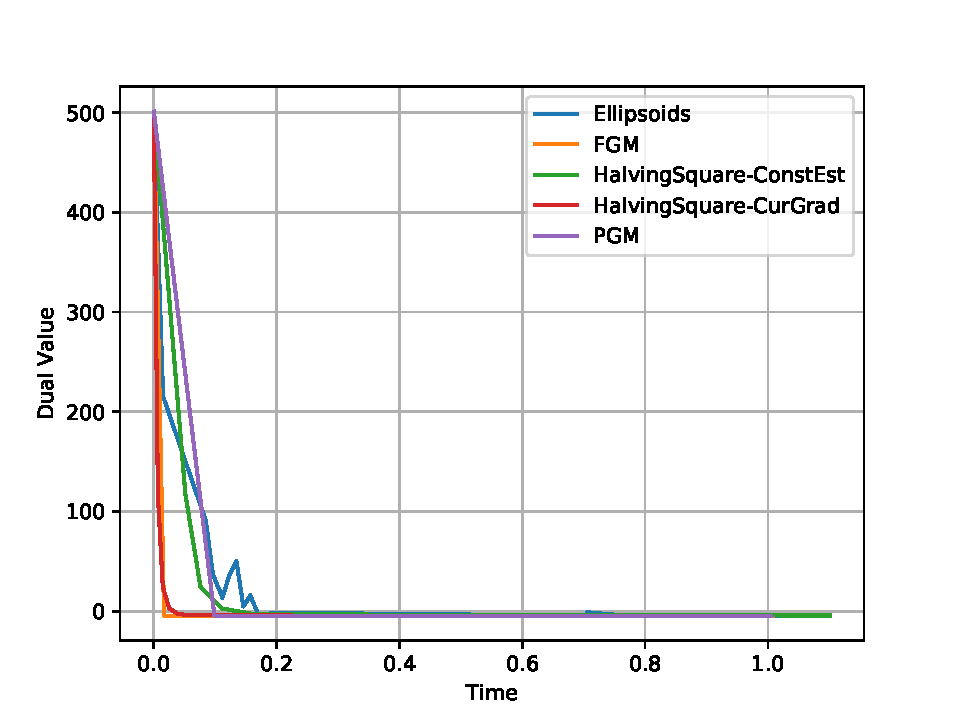
\includegraphics[width=0.25\linewidth]{../Tests/Images/100_1e-03.pdf} \label{100_3} }  
\hspace{2ex}
\subfigure[]{
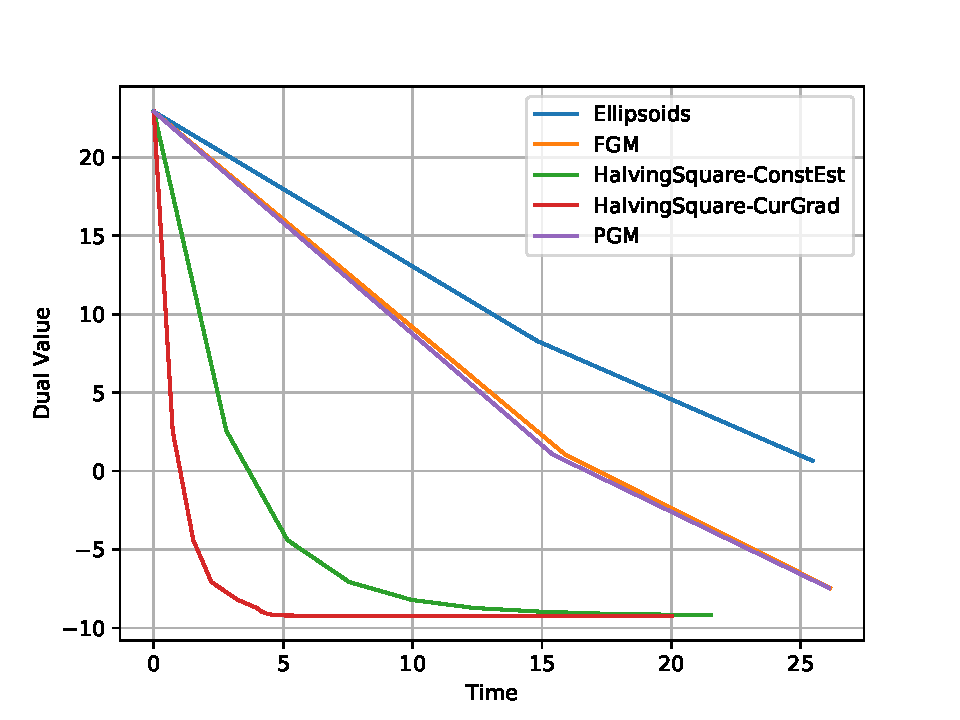
\includegraphics[width=0.25\linewidth]{../Tests/Images/100_1e-10.pdf} \label{100_10} }
\vspace{2ex}
\subfigure[]{
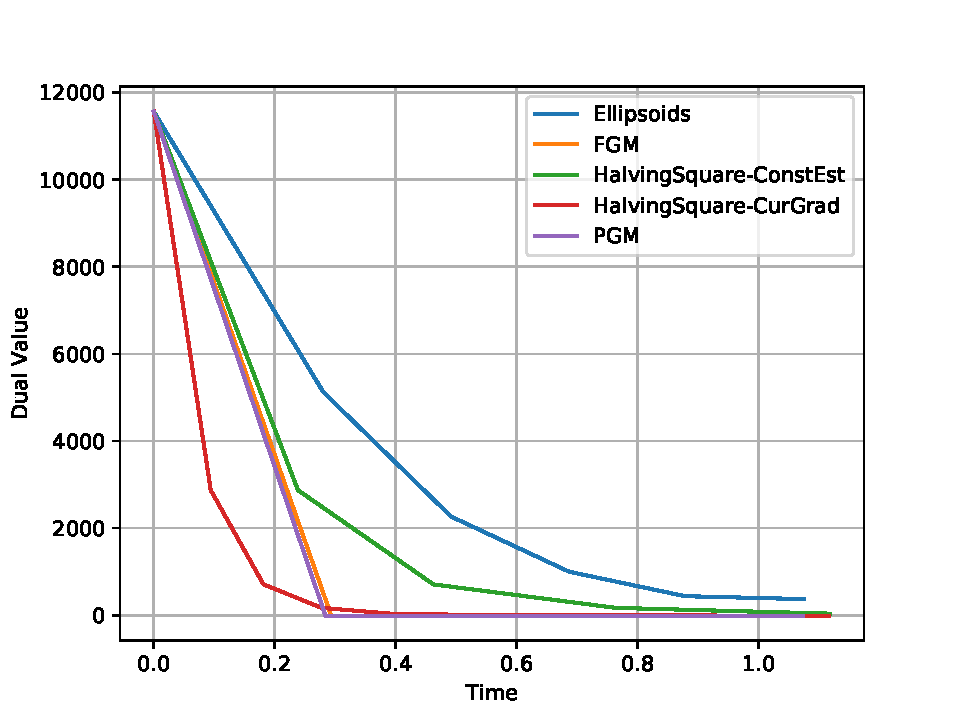
\includegraphics[width=0.25\linewidth]{../Tests/Images/1000_1e-03.pdf} \label{1000_3} }  
\hspace{2ex}
\subfigure[]{
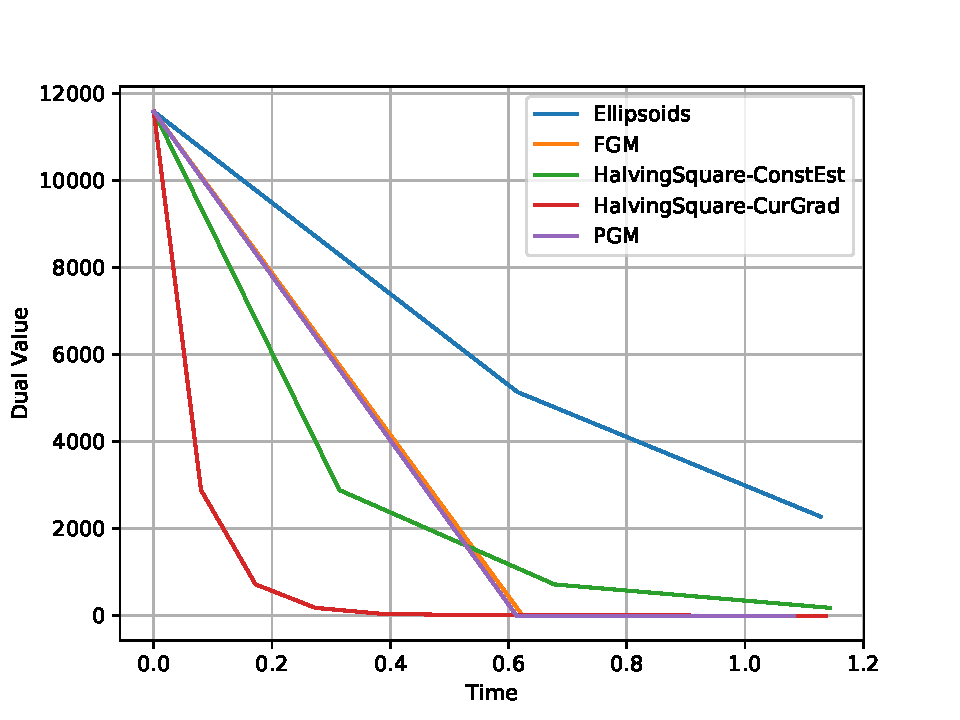
\includegraphics[width=0.25\linewidth]{../Tests/Images/1000_1e-10.pdf} \label{1000_10} }
\vspace{2ex}
\subfigure[]{
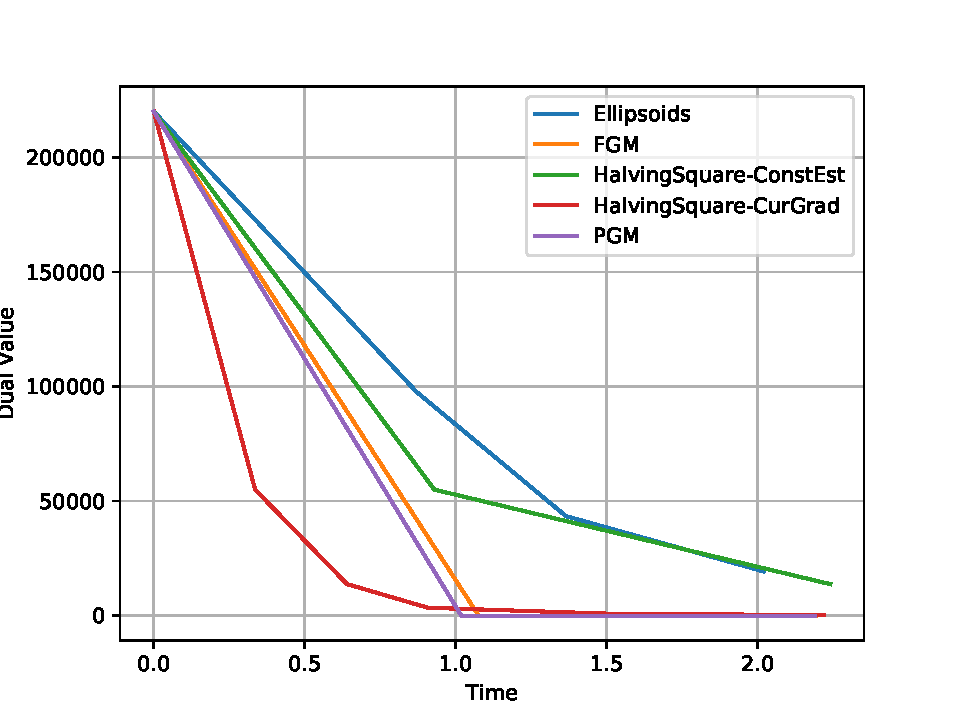
\includegraphics[width=0.25\linewidth]{../Tests/Images/10000_1e-03.pdf} \label{10000_3} }  
\hspace{2ex}
\subfigure[]{
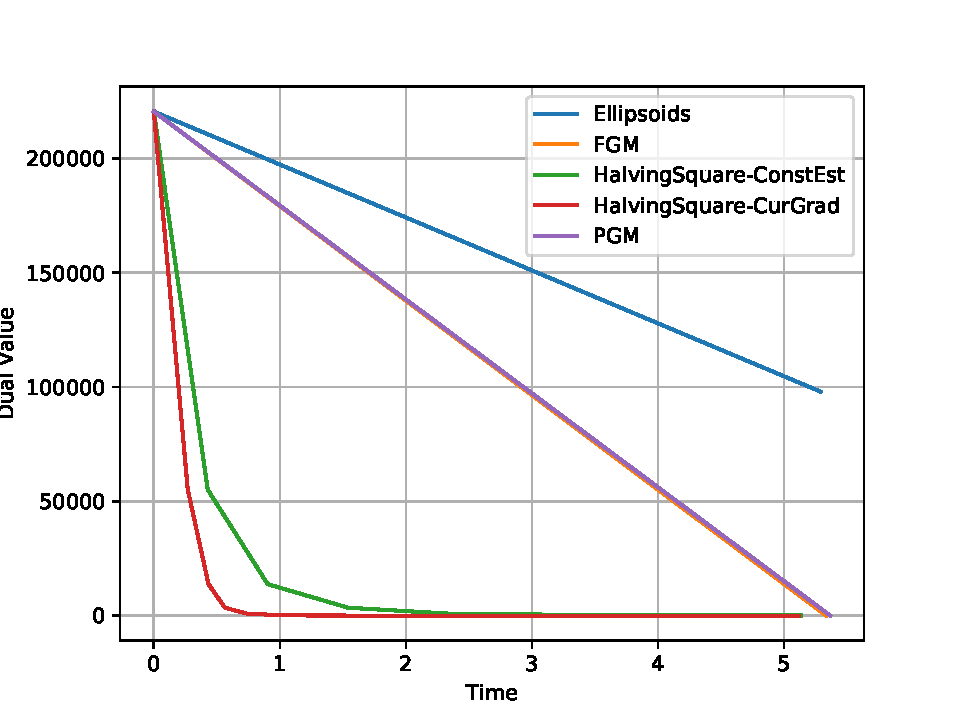
\includegraphics[width=0.25\linewidth]{../Tests/Images/10000_1e-10.pdf} \label{10000_10} }
\hspace{2ex}
\caption{Comparison of different on inexact methods for task with different dimension $N$ and for different required accuracy $\epsilon$: \subref{100_3} $N=100,\epsilon=10^{-3}$; \subref{100_10} $N=100,\epsilon=10^{-10}$; \subref{1000_3} $N=1000,\epsilon=10^{-3}$; \subref{1000_10} $N=1000,\epsilon=10^{-10}$; \subref{10000_3} $N=10000,\epsilon=10^{-3}$; \subref{10000_10} $N=10000,\epsilon=10^{-10}$. } \label{fig:image}
\end{figure}

Let's compare our method with inexact ellipsoid method and gradient methods (PGM and FGM) with $(\delta, L,\mu)$ oracle (see previous subsection \ref{Inexact}) on a dual task.

For to find $\textbf{x}(\lambda)$ we will use gradient descent. There are theoretical result that can help to manange distance $\|\textbf{x}_k-\textbf{x}^*\|$ from optimal point to its current approximation. In particular, there are following results:
\begin{itemize}
\item If $f$ is a convex function with $L$-Lipschitz continious gradient then gradient descent with step $\alpha_k = \frac{1}{L}$ converges with speed
$$\|f(\textbf{x}_k)-f(\textbf{x}^*)\|\leq \frac{\|\textbf{x}_0-\textbf{x}^*\|}{k+4}$$
\item If $f$ is a $\mu$-strong convex function with $L$-Lipschitz continious gradient then gradient descent with step $\alpha_k = \frac{1}{L+\mu}$ converges with speed
$$\|f(\textbf{x}_k)-f(\textbf{x}^*)\|\leq \left(\frac{M-1}{M+1}\right)^kL\|\textbf{x}_0-\textbf{x}^*\|,$$
where $M =\frac{L}{\mu}$.
\end{itemize}

The proves for this statements one can find in many books of optimization, for example, in the book \cite{Polyak}.

We will use functions where $\mu$ is small enough. Therefore, our method for calculating $\textbf{x}(\lambda)$ will converge to solution according to the first estimate.

For all inexact method we will calculate $\textbf{x}(\lambda)$ with such accuracy as the method will converge to the solution with same for all methods accuracy $\epsilon$. For PGM, FGM and ellipsoids methods we will calculate $\textbf{x}(\lambda)$ with accuracy $\frac{\epsilon}{2}$ on function. For our method with the both strategies we will calculate $\textbf{x}(\lambda)$ untill the conditions from the \ref{dual} is approached.


We consider the following prime task:

\begin{gather}
\label{prime}
f(\textbf{x}) = \ln \left(1+\sum_{k=1}^ne^{\alpha x_k}\right) + \beta\|\textbf{x}\|_2^2\rightarrow \min\limits_{\textbf{x}\in \mathbb{R}^N}\\
g_k(\textbf{x}) = \langle \textbf{b}_k, \textbf{x}\rangle+c_k\leq0, k = \overline{1,m}\\
\end{gather}

It is task of minimization the LogSumExp-function with $l2$-regularization. The regularization parameter $\beta$ determines strong convexity of our task and in the tests one takes $beta=0.1$. The $N$ is diminsionality of primal task and is determined for different tests below. The parameter $\alpha$ is equal to 1. The parameters $c_k$ are equal to 1 too. The vectors $\{b_k\}_{k=1}^m$ are generated randomly for the each test. The $m$ is equal to dimensionality of dual task and in the current case is equal to 2.

The LogSumExp-problem is $L$-Lipschitz continious function with $M$-Lipschitz continious gradient where $L=1$ and $M=\alpha$. Therefore:
$$L_f = \alpha+2\beta R, M_f = \alpha^2 + 2\beta,$$
$$\mu_f = 2\beta,$$
where $R=\|\textbf{x}_0-\textbf{x}^*\|$ is the size of initial approximation. The functions $g_k$ are $L_k$-Lipschitz continious where $L_k=\|b_k\|$. 

We introduce the following notation:

\begin{equation}
\label{phi}
\phi(\lambda_1, \lambda_2) = -\min\limits_{\textbf{x}\in \mathbb{R}^N}\left(f(\textbf{x}) +\lambda_1 g_1(\textbf{x}) +\lambda_2g_2(\textbf{x})\right)
\end{equation}

In such notations the dual task for the task \ref{prime} looks like:

\begin{gather}
\phi(\lambda_1, \lambda_2) \rightarrow \min\limits_{\lambda_1, \lambda_2}\\
\text{s.t}\, \lambda_1, \lambda_2 \geq 0
\end{gather}
 
Obviously, $\min\limits_{\textbf{x}}f(\textbf{x}) \geq 0$. Therefore, according to \ref{restr:dual} we can add following conditions on the dual variables:

$$|\lambda_k| \leq \lambda_{\text{max}}=\frac{f(\overline{\textbf{x}})}{\gamma}, k=1,2$$

And we have following task:

$$\phi(\lambda_1, \lambda_2) \rightarrow \min_{0\leq\lambda_k\leq\lambda_{max}}$$

Calculating of function and derivatave value for such task was discussed in the section \ref{details}.

We can see on \ref{fig:image} the following results. Firstly, the halving square method with provided in this work strategy \textbf{CurGrad} are the fastest method in the most tests tests. This method can be slower than other inexact methods if dimensional of primal task is small or $\epsilon$ is big. In particular, this strategy is faster than strategy with constant estimate provided in \cite{Ston_Pas}. It proves that provided by Nesterov method with strategy through gradient is the best method for to solve two dimensional dual task of minimization. Secondly, the gain of this strategy in comparison with other method is increase when the required $\epsilon$ decrease. This fact demonstrated important advantange of this strategy: it does not depend on required accuracy strongly. So, this method with constant estimate has strong dependity on it because there is this accuracy in the constant estimate, PGM and inexact ellipsoid method require that the $x(\lambda)$ is found with accuracy depended on $\epsilon$. But halving square with ellipsoid method has not such dependety.
\section{Conclusion}

We discussed and proved that this method converges to the solution for smooth convex functon. Moreover, in the \cite{Ston_Pas} there is conterexample when the problem is non-smooth and we can not to converge to the solution with the accuracy on function better than a constant.

After it we discussed different strategy for one-dimensional task. Two strategies were considered. The both suggest to use stop conditions that are met when the current approximation is "very near" to the segment's solution. The first compares the distance between them with derivative value in accurate segment's solution but the second compares it with derivative value in approximation. In the experiment the first has a little better result but it can not be used for real task. The second strategy using derivative value in current approximation is significantly better then constant estimate and does not depend on required accuracy.

But all this strategy are good when the derivative value is high enough. But when the segment is near to the global solution this value will be small. Therefore one needs to make a lot of iterations on segment. For to avoid it we consider additional stop condition for global task on square when in current approximation the derivative value is near to zero.

The most steps of methods assumped that derivative can be calculated accurately. But the main method purpose is to solve dual problems and for it one can not usually calculate it so. That's why we consider different modifications of this method for to solve such problems. The important moment is we don't add some dependence on initial required accuracy in the modificated method.

Finally, we compared our method with new strategy for dual problem to prime LogSumExp problem with two linear constaints with our method with strategy using the constant estimate, primal gradient method and fast gradient method with $(\delta, L, \mu)$ -oracle and with inexact ellipsoids methods. The Halving Square Method is the fastest of them for enough high dimension (more 100) and for enough high required solution ($1e-3$ and more).

\newpage
\begin{thebibliography}{3}
\bibitem{task}
Gasnikov A.  Universal gradient descent // MIPT --- 2018, 240 p.
\bibitem{Ston_Pas}
Pasechnyk D.A., Stonyakin F.S.  One method for minimization a convex Lipchitz continuous function of two variables on a fixed square // arXiv.org e-Print archive. 2018. – URL: \href{https://arxiv.org/pdf/1812.10300.pdf}{https://arxiv.org/pdf/1812.10300.pdf}
\bibitem{Nesterov}
Nesterov U.E.  Methods of convex optimization // M.MCNMO --- 2010, 262 p.
\bibitem{conda}
Anaconda[site]. At available: \href{https://www.anaconda.com}{https://www.anaconda.com}
\bibitem{DDR-theorem}
Danskin, J.M.: The theory of Max-Min, with applications. J. SIAM Appl. Math.14(4) (1966)
\bibitem{Stonykin}
Fedor S. Stonyakin, Mohammad S. Alkousa, Alexander A. Titov,and Victoria V. Piskunova1 On Some Methods for Strongly Convex Optimization Problems with One Functional Constraint // ...
\bibitem{PGM}
Olivier Devolder Exactness, Inexactness and Stochasticityin First-Order Methods for Large-ScaleConvex Optimization // UCL --- 2013,
\bibitem{Ellipsoids}
Need Reference To Book with Inexact Ellipsoids
\bibitem{Polyak}
B.T. Polyak. The Introduction to Optimization // Moscow, Science - 1983
\bibitem{my_git}
Repository with code: \href{https://github.com/ASEDOS999/Optimization-Halving-The-Square}{https://github.com/ASEDOS999/Optimization-Halving-The-Square}
\end{thebibliography}
\end{document}
